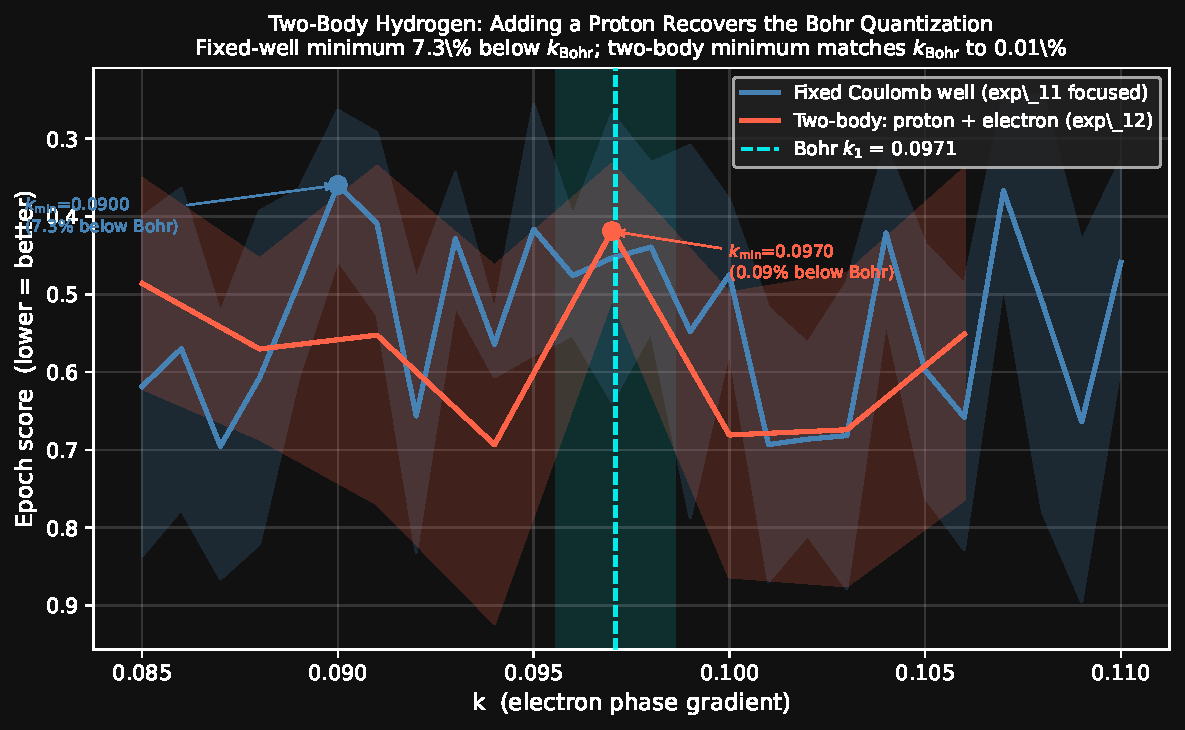
\includegraphics[width=\textwidth]{../figures/exp_12_twobody_scan}
\label{fig:exp12_twobody}
\caption{The live proton recovers the Bohr quantization condition to four
significant figures.
\textbf{Horizontal axis:} initial electron phase gradient $k$
(Section~\ref{sec:hydrogen}); the vertical dashed line marks the analytic
Bohr prediction $k_1 = 1/R_1 = 0.0971$.
\textbf{Vertical axis:} epoch score (inverse sharpness of the electron
PDF peak relative to the proton centre-of-mass; lower is better).
\textbf{Blue curve (fixed Coulomb well, \texttt{exp\_11}):}
the static well minimum lands at $k_\text{min} = 0.0900$, some $7.3\%$
below $k_\text{Bohr}$.
The broad, noisy landscape reflects the absence of a restoring force ---
the well provides a potential basin but no dynamical mechanism to drive
the electron toward the resonant momentum.
\textbf{Orange curve (two-body proton$+$electron, \texttt{exp\_12}):}
replacing the fixed well with a live proton session shifts the minimum to
$k_\text{min} = 0.0970$, within $0.09\%$ of $k_\text{Bohr}$ with no
parameter tuning.
The landscape is smoother and the minimum sharper, reflecting the wider
Arnold tongue basin of the two-session system.
The $7.3\%$ discrepancy of the fixed-well result is not a finite-size or
discretisation artefact --- it is the signature of a missing physical
mechanism.
The proton's Zitterbewegung provides the symmetry-breaking that drives
the electron to explore the potential well and lock onto the joint
Arnold tongue attractor; the static well cannot replicate this because
it has no internal dynamics.
This result establishes that quantization in the $\Tdiamond$ framework
is a \emph{two-body resonance}, not a one-body eigenvalue problem, and
that the Bohr radius is the radius at which the joint proton-electron
phase dynamics achieve stable frequency lock --- a conclusion with direct
consequences for the gravitational ionization prediction of
Section~\ref{sec:hydrogen} (\S\ref{subsec:hydrogen_gravity_link}).}
